% For this appendix, undo tufte-latex's big margin
\newgeometry{left=1in,right=1in,bottom=1.5in,textwidth=6.5in,marginparsep=0pc,marginparwidth=0pc}
% Recalculate fancy header/footer after geometry change (otherwise page numbers are misplaced)
\fancyhfoffset[E,O]{0pt}

\chapter{Appendix Figures}

\begin{figure*}[p]
  \centering
  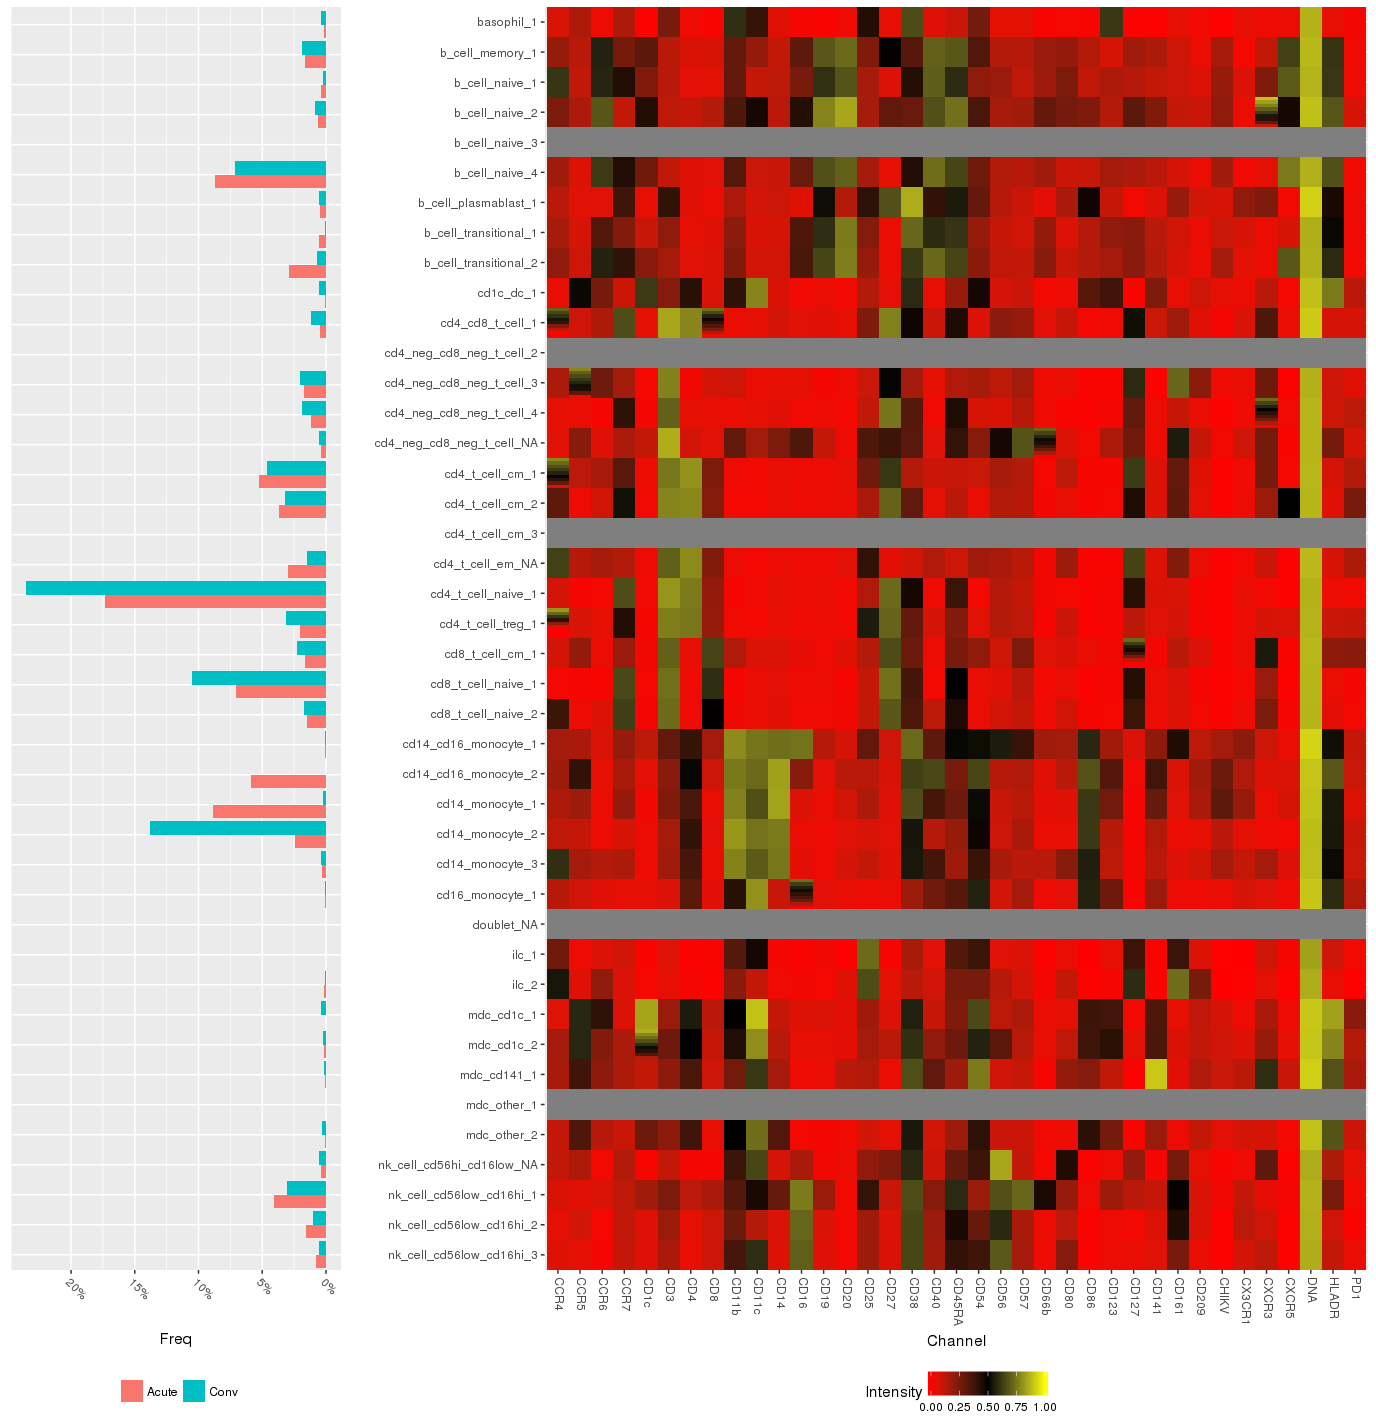
\includegraphics[width=\textwidth]{chap5/fig_S1a_MHL_example_1800}
  \fullwidthlabelcaption{fig:mhl_example}{Example output of \texttt{MetaHybridLouvain} for a representative paired CyTOF sample}{
  \textbf{Example output of \texttt{MetaHybridLouvain}} for the representative sample used in Figure \ref{fig:nodlabel_diag}, Figure \ref{fig:mhl_visne}, and \ref{fig:chikv_visne}. At left, frequencies for each sub-community at each timepoint, and at right, mini-heatmaps of channel values for each sub-community (plotted within each row). As expected, sub-communities generally show similar values among all channels for their constituent events, with some exceptions (vertical gradients within mini-heatmaps). \emph{Continued in Figure \ref{fig:mhl_example_cont}.}
  }
\end{figure*}

\begin{figure*}[p]
  \centering
  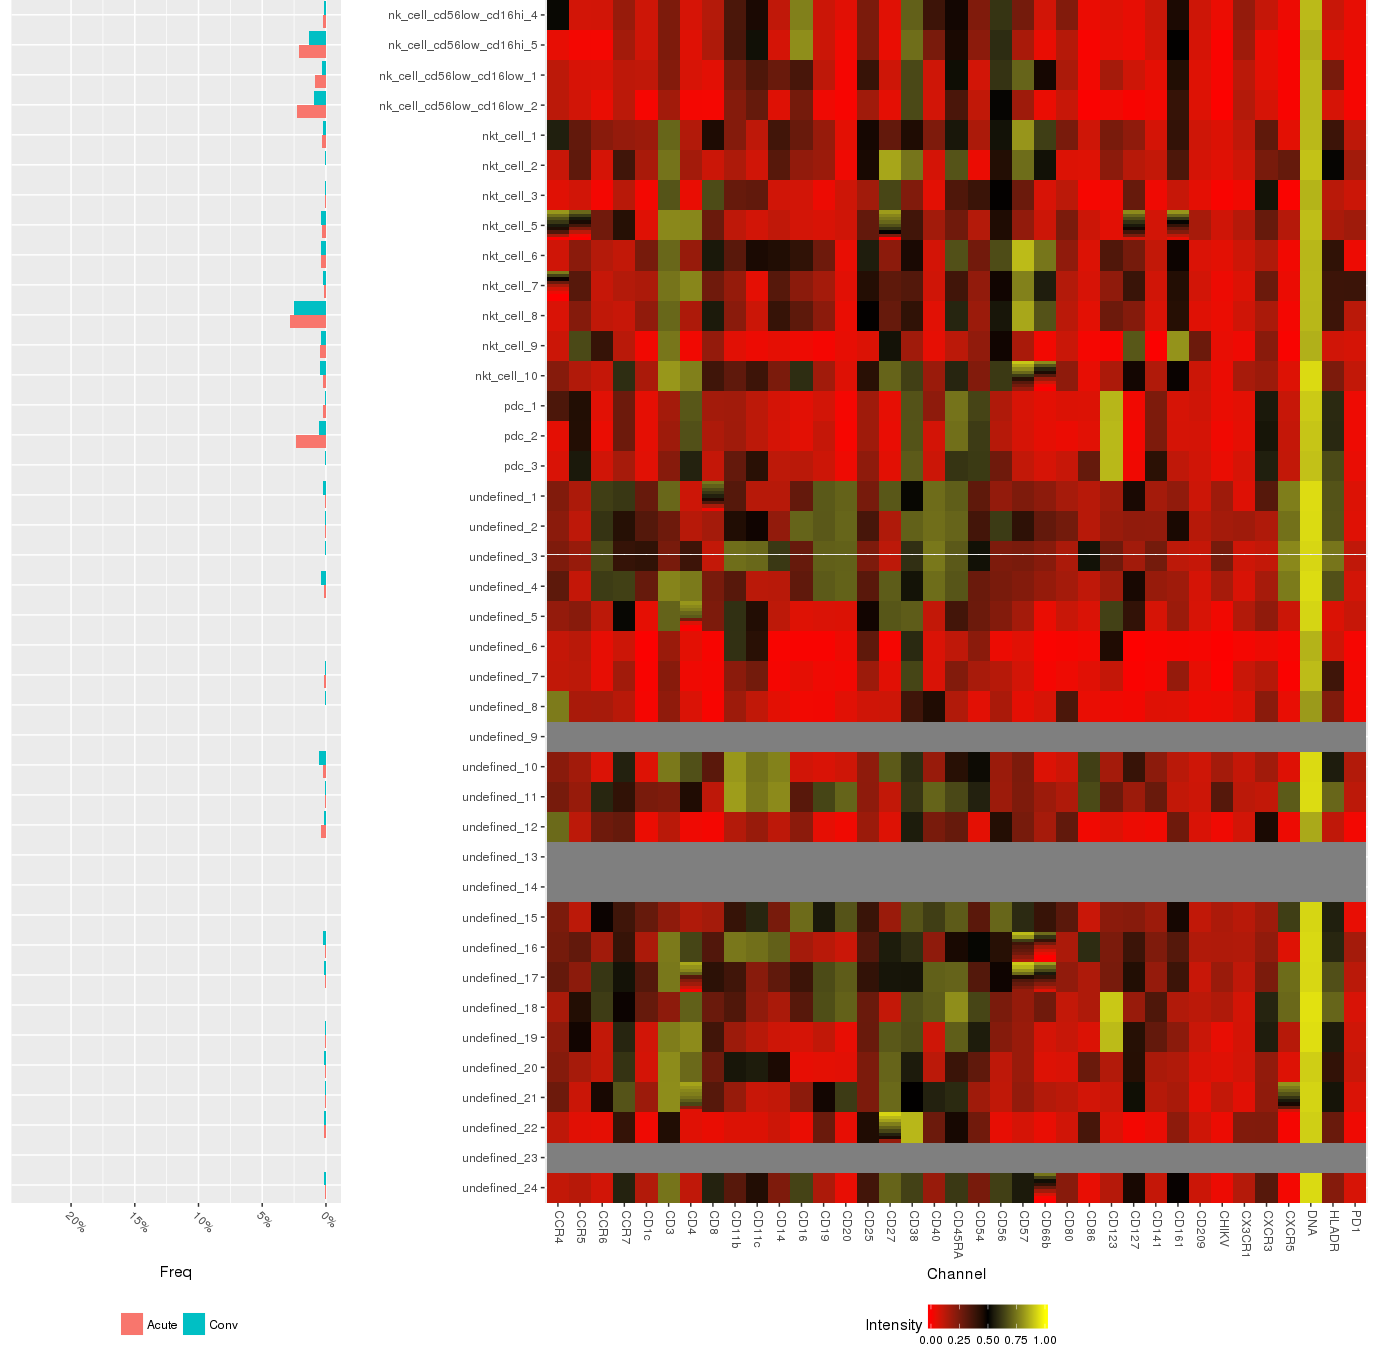
\includegraphics[width=\textwidth]{chap5/fig_S1b_MHL_example_1800}
  \fullwidthlabelcaption{fig:mhl_example_cont}{Example output of \texttt{MetaHybridLouvain} for a representative paired CyTOF sample, continued}{
  \textbf{Continuation of example output of \texttt{MetaHybridLouvain}} for the representative sample used in Figure \ref{fig:nodlabel_diag}, Figure \ref{fig:mhl_visne}, and \ref{fig:chikv_visne}. At left, frequencies for each sub-community at each timepoint, and at right, mini-heatmaps of channel values for each sub-community (plotted within each row). As expected, sub-communities generally show similar values among all channels for their constituent events, with some exceptions (vertical gradients within mini-heatmaps). \emph{Continued from Figure \ref{fig:mhl_example}.}
  }
\end{figure*}

\begin{figure*}[p]
  \centering
  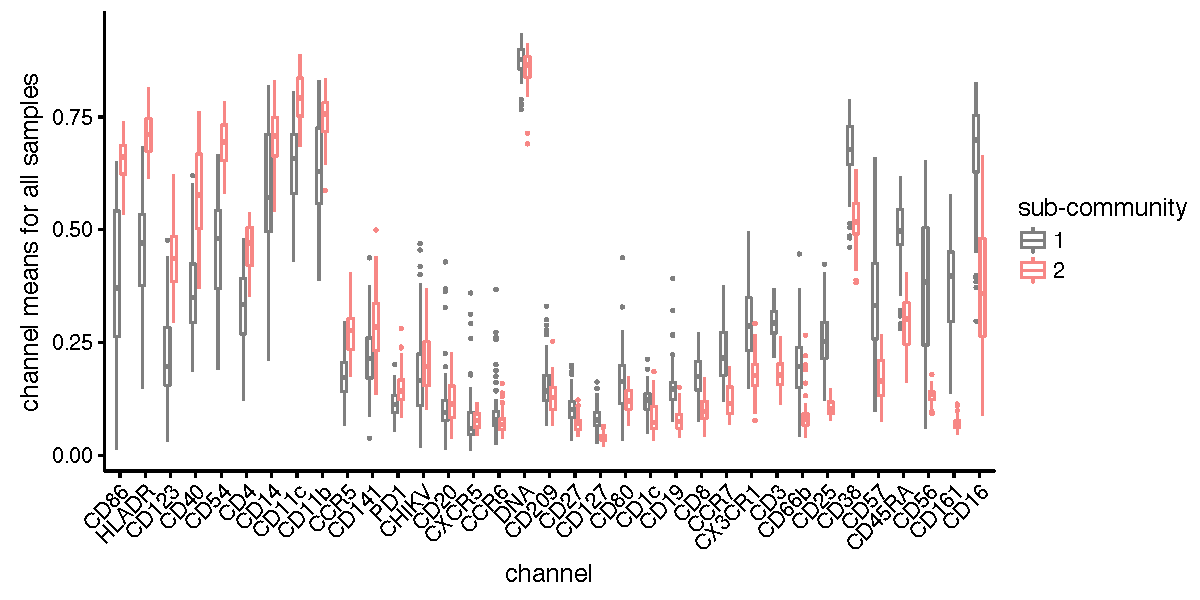
\includegraphics[width=\textwidth]{chap5/fig_S3_cd14c16_monocytes_subpop_differences}
  \fullwidthlabelcaption{fig:cd14cd16_channel_diffs}{Differences in per-sample channel means between two CD14\sups{+}CD16\sups{+} sub-communities identified by \texttt{MetaHybridLouvain}.}{
  \textbf{Differences in per-sample channel means between two CD14\sups{+}CD16\sups{+} sub-communities identified by \texttt{MetaHybridLouvain}.} 1 corresponds with the “intermediate” CD14\sups{++}CD16\sups{+} phenotype, while 2 corresponds with the “nonclassical” CD14\sups{+}CD16\sups{++} phenotype. The X axis is filtered to only the channels with differences significant at FDR < 0.05, and ordered from differences where sub-community 1 < 2 on the left to sub-community 1 > 2 on the right.
  }
\end{figure*}

%fig_S3_cd14c16_monocytes_subpop_differences

%fig_S6_cytof.MHL.subpop_channelmeans.cd14

%fig_S10_nonsig_luminex

%fig_S11_corrplot.luminex-cytof.all.both-times
%fig_S12_corrplot.luminex-cytof.all.acute
%fig_S13_corrplot.luminex-cytof.all.conv

%fig_S15_corrplot.luminex-mrna.cytokines.both
%fig_S16_corrplot.luminex-mrna.cytokines.acute-minus-conv

%fig_S18_hsa04062.timepoint.log2fc
%fig_S19_hsa04620.timepoint.log2fc
%fig_S20_hsa04622.timepoint.log2fc
%fig_S21_hsa04630.timepoint.log2fc
%fig_S22_hsa04668.timepoint.log2fc
%fig_S23_hsa05164.timepoint.log2fc

%fig_S26_cytof-luminex-genemodules

% Restore the geometry of tufte-latex's big right margin
\restoregeometry
% Restore tufte-latex's fancy header/footer offsets
\tuftefancyhfoffset

\clearpage
\newpage

% Recalculate fancy header/footer after geometry change (otherwise page numbers are misplaced)
%\fancyhfoffset[E,O]{0pt}
